\documentclass{beamer}
\usepackage[utf8]{inputenc}
\usepackage[]{amsmath}
\usepackage{graphicx}
\usepackage{physics}
\usepackage{subcaption} % package pour faire des subfigures
\usepackage{multirow} % package pour multirow/multicolumn
\usepackage{booktabs} % package pour top/mid/bottom rule
\usepackage{tcolorbox} % toujours plus de boites
\usepackage[backend=biber]{biblatex}


\addbibresource{Biblio_dbl_quantum.bib}

%\bibliographystyle{stylename}
%\bibliography{Biblio_dbl_quantum}

\title{Dipolar interactions in dense ensembles of Nitrogen-Vacancy centers}
\author{Clément Pellet-Mary, Maxime Perdriat, Gabriel Hétet}
\date{Nano-optics group}

\mode<presentation> {\usetheme{Rochester}}

\begin{document}
\begin{frame}
\maketitle
\centering
\includegraphics[scale=.2]{Nitrogen-vacancy_center}
\end{frame}
%\begin{frame}{Outline}
%\tableofcontents
%\end{frame}
%\section{Physics of the NV center}
\begin{frame}{Team main activities}
\centering
\includegraphics[width=\textwidth,height=0.9\textheight,keepaspectratio]{Slide activités}
\end{frame}

\begin{frame}{Optical properties of NV$^-$ centers}
\centering
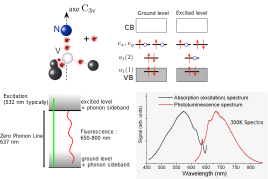
\includegraphics[width=\textwidth,height=0.9\textheight,keepaspectratio]{slide_NV_optical}
\end{frame}
%\begin{frame}{NV$^-$ center electronic structure}
%\centering
%\includegraphics[width=\textwidth,height=0.9\textheight,keepaspectratio]{NV_8_niveaux_1}
%\end{frame}
%\begin{frame}{NV$^-$ center electronic structure}
%\centering
%\includegraphics[width=\textwidth,height=0.9\textheight,keepaspectratio]{NV_8_niveaux_2}
%\end{frame}
\begin{frame}{NV$^-$ center electronic structure}
\centering
\includegraphics[width=\textwidth,height=0.9\textheight,keepaspectratio]{NV_8_niveaux_3}
\end{frame}
\begin{frame}{NV center spin sub-levels}
\centering
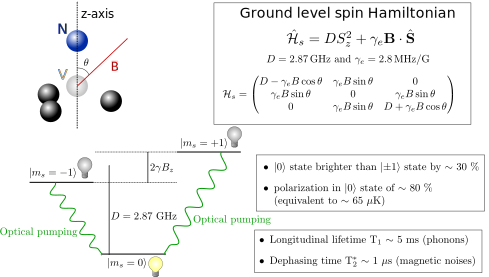
\includegraphics[width=\textwidth,height=0.9\textheight,keepaspectratio]{slide_3_niveaux}
\end{frame}
\begin{frame}{Optically Detected Magnetic Resonance (ODMR)}
\centering
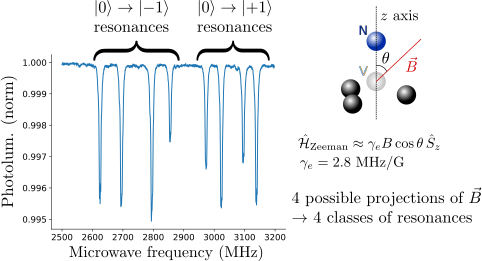
\includegraphics[width=\textwidth,height=0.9\textheight,keepaspectratio]{slide ODMR}
\end{frame}
\begin{frame}{Modification of the spin $T_1$ with dense ensemble}
\centering
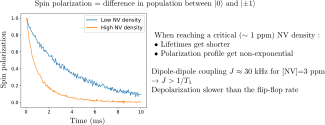
\includegraphics[width=\textwidth,height=0.9\textheight,keepaspectratio]{slide_T1_1}
\end{frame}
\begin{frame}{Modification of the spin $T_1$ due to resonant dipole coupling}
\centering
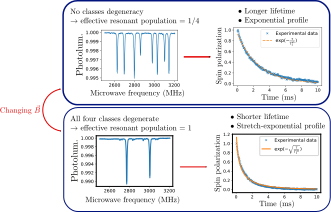
\includegraphics[width=\textwidth,height=0.9\textheight,keepaspectratio]{slide_T1_2}
\end{frame}
\begin{frame}{Dipole-dipole coupling in zero magnetic field}
\centering
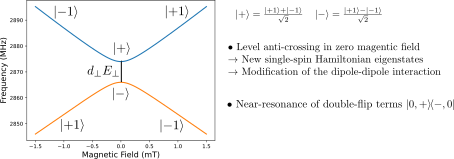
\includegraphics[width=\textwidth,height=0.9\textheight,keepaspectratio]{Slide zero field}
\end{frame}
\begin{frame}{Conclusion}
\begin{itemize}
\item The NV$^-$ center is an optically active defect in diamond which allows an optical control and readout of its spin state.
\bigskip
\item The depolarization of the spins is modified in dense ensemble due to dipole-dipole coupling.
\bigskip
\item This effect is even stronger in zero-magnetic field.
\end{itemize}
\end{frame}
\begin{frame}{Bonus : Magnetometry in zero magnetic field}
\centering
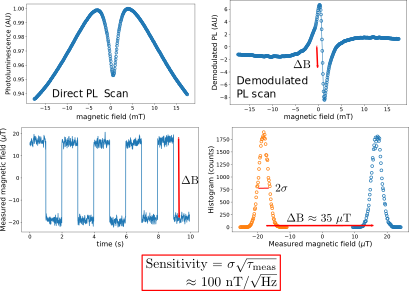
\includegraphics[width=\textwidth,height=0.9\textheight,keepaspectratio]{Slide_magneto}
\end{frame}

\end{document}